\section{System APIs}



\begin{frame}
  \frametitle{Threads API}

  \begin{itemize}
  \item Lifecycle management
    \begin{itemize}
    \item Creation
    \item Destruction
    \end{itemize}
  \item Synchronization
    \begin{itemize}
    \item Lifecycle synchronization
    \item Share resources
    \item Share work
    \end{itemize}
  \item Tuning
    \begin{itemize}
    \item Scheduling
    \item Stack
    \item Signals
    \item ...
    \end{itemize}
  \end{itemize}
\end{frame}









\subsection{POSIX Threads}
\label{subsec:pthreads}



\begin{frame}
  \frametitle{Introducing the POSIX Threading API}

  \begin{itemize}
  \item \emph{pthreads} for short
    \begin{itemize}
    \item \emph{pthread\_xxx} functions
    \item Man pages: \textbf{man 7 pthreads}
    \end{itemize}
  \item Primitives
    \begin{itemize}
    \item Lifecycle management
    \item Synchronization
    \item Tuning
    \end{itemize}
  \end{itemize}
\end{frame}

\begin{frame}
  \frametitle{Why the low-level API ?}

  \begin{itemize}
  \item The more you know
    \begin{itemize}
    \item Used in a lot of code
    \item Precise documentation
    \item System semantic and behavior
    \end{itemize}
  \item More control
  \item Not everything is wrapped
  \item Access to non-portable features
  \end{itemize}
\end{frame}


\begin{frame}
  \frametitle{Lifecycle management}

  \begin{itemize}
  \item Creation
    \begin{itemize}
    \item Process creation
    \item \emph{pthread\_create()} with a function pointer
    \end{itemize}
  \item Destruction
    \begin{itemize}
    \item The thread function returns
    \item \emph{pthread\_exit()} exits the current thread
    \item \emph{pthread\_cancel()} ask for another thread to exit
    \end{itemize}
  \end{itemize}
\end{frame}



\begin{frame}
  \frametitle{Cancellation}

  \begin{itemize}
  \item \emph{pthread\_cancel()} sends cancellation request
  \item Thread can configure their policy (\emph{pthread\_setcanceltype()})
    \begin{itemize}
    \item Asynchronous: Exit ASAP
    \item Deferred: Exit on a cancellation point
    \end{itemize}
  \item Can be disabled with \emph{pthread\_setcancelstate()}
  \item Cleanup handlers with \emph{pthread\_cleanup\_push}
  \item Cancellation points:
    \begin{itemize}
    \item \emph{pthread\_testcancel()}
    \item Certain syscalls: see ``man 7 pthreads''
    \end{itemize}
  \end{itemize}
\end{frame}



% XXX: Add some examples


\begin{frame}
  \frametitle{Synchronization}

  \begin{itemize}
  \item MUTual EXclusions (aka mutex or lock)
    \begin{itemize}
    \item Thread can acquire/release it
    \item Only 1 thread can acquire it at the time
    \item Helps protect shared resources
    \end{itemize}
  \item RW Locks
    \begin{itemize}
    \item Acquired for Read OR Write
    \item Multiple reader OR one writer at the time
    \end{itemize}
  \item Conditions / Signals
    \begin{itemize}
    \item Wait for a condition to happen
    \item Signal (awake threads) when a condition happen
    \end{itemize}
  \item Barriers
    \begin{itemize}
    \item Wait for \emph{N} other threads to reach a certain point
    \end{itemize}
  \end{itemize}

\end{frame}


\begin{frame}[fragile]{Mutex}

  \begin{itemize}
  \item Helps protect a shared resource from concurrent access.
  \item Lifecycle
    \begin{itemize}
    \item \emph{pthread\_mutex\_init()}
    \item \emph{pthread\_mutex\_destroy()}
    \item \verb+pthread_mutex_t mutex = PTHREAD_MUTEX_INITIALIZER;+
    \end{itemize}
  \item Lock
    \begin{itemize}
    \item \emph{pthread\_mutex\_lock()}
    \item \emph{pthread\_mutex\_timedlock()}
    \item \emph{pthread\_mutex\_trylock()}
    \end{itemize}
  \item Unlock: \emph{pthread\_mutex\_unlock()}
  \end{itemize}
\end{frame}


\begin{frame}[fragile]
  \frametitle{RW Locks}

  \begin{itemize}
  \item Helps protect a shared resource from concurrent access.
  \item For \emph{read-mostly} data
  \item Lifecycle
    \begin{itemize}
    \item \emph{pthread\_rwlock\_init()}
    \item \emph{pthread\_rwlock\_destroy()}
    \item \verb+pthread_rwlock_t rwl = PTHREAD_RWLOCK_INITIALIZER;+
    \end{itemize}
  \item Lock as a writer:
    \begin{itemize}
    \item \emph{pthread\_rwlock\_wrlock()}
    \item \emph{\_trywrlock()},  \emph{\_timedwrlock()}
    \end{itemize}
  \item Lock as a reader:
    \begin{itemize}
    \item \emph{pthread\_rwlock\_rdlock()}
    \item ...
    \end{itemize}
  \item Unlock: \emph{pthread\_rwlock\_unlock()}
  \end{itemize}
\end{frame}


\begin{frame}
  \frametitle{Conditions}

  \begin{itemize}
  \item 1-n thread(s) wait(s) on a condition
  \item Another thread wakes one or all waiting thread(s)
  \item Requires a mutex
  \item API calls:
    \begin{itemize}
    \item \emph{pthread\_cond\_init()} and \emph{pthread\_cond\_destroy()}
    \item Wait: \emph{\_cond\_wait()} and \emph{\_cond\_timedwait()}
    \item Wake one: \emph{\_cond\_signal()}
    \item Wake all: \emph{\_cond\_broadcast()}
    \end{itemize}
  \end{itemize}
\end{frame}


\begin{frame}
  \frametitle{Barriers}

  \begin{itemize}
  \item A barrier is initialized with an int ``N''.
  \item Threads may \emph{wait} on the barrier.
  \item When ``N'' threads are waiting, they're all resumed.
  \item One thread get a special value returned, the other get 0.
  \item API calls:
    \begin{itemize}
    \item \emph{pthread\_barrier\_init()} and \emph{\_destroy()}
    \item \emph{pthread\_barrier\_wait()}
    \end{itemize}
  \item != Memory barriers
  \end{itemize}
\end{frame}


\begin{frame}
  \frametitle{Spinlocks}

  \begin{itemize}
  \item Busy-wait based locks
    \begin{itemize}
    \item Avoid context switches
    \item Waste CPU Time
    \end{itemize}
  \item Good for short lived locks
  \item API Calls:
    \begin{itemize}
    \item \emph{pthread\_spin\_init} and \emph{\_destroy}
    \item \emph{\_lock()} and \emph{\_unlock()}
    \end{itemize}
  \end{itemize}
\end{frame}


\begin{frame}
  \frametitle{Utils}

  \begin{itemize}
  \item Wait for a thread to terminate: \emph{pthread\_join()}
  \item Get called before/after fork: \emph{pthread\_atfork()}
  \item Get the current thread: \emph{pthread\_self()}
  \item Compare threads: \emph{pthread\_equals()}
  \item Call a function once per process: \emph{pthread\_once()}
  \item Relinquish the CPU: \emph{pthread\_yield()} or \emph{sched\_yield()}
  \end{itemize}
\end{frame}

\begin{frame}
  \frametitle{Thread Local Storage}

  \begin{itemize}
  \item Thread specific pointers
  \item Non thread-safe library (codec, interpreter, ...)
  \item API Calls:
    \begin{itemize}
    \item Create a key: \emph{pthread\_key\_create()}
    \item \emph{pthread\_key\_destroy()}
    \item Store a pointer for key/thread: \emph{pthread\_setspecific()}
    \item Get the pointer: \emph{pthread\_getspecific()}
    \end{itemize}
  \end{itemize}
\end{frame}

\begin{frame}[fragile]
  \frametitle{TLS Example}

  \begin{minted}[fontsize=\scriptsize]{c}
    static pthread_key_t key;
    static pthread_once_t key_once = PTHREAD_ONCE_INIT;

    static void make_key() {
      (void) pthread_key_create(&key, NULL);
    }

    func() {
      void *ptr;

      (void) pthread_once(&key_once, make_key);
      if ((ptr = pthread_getspecific(key)) == NULL) {
        ptr = malloc(OBJECT_SIZE);
        // ...
        (void) pthread_setspecific(key, ptr);
      }
      // ...
    }
  \end{minted}
\end{frame}




\subsection{C++ 11}
\label{subsec:cpp11}

\begin{frame}
  \frametitle{threading in std::}

  \begin{itemize}
  \item C++11 adds threading support in the stdlib
  \item Clean C++
  \item Support portable behaviors and primitives
  \item Supported by most compilers/stdlib:
    \begin{itemize}
    \item gcc/libstd++
    \item clang/libc++
    \item MSVC 2012+
    \item icc: meh !
    \end{itemize}
  \item boost::thread is close-enough
  \end{itemize}
\end{frame}


\begin{frame}
  \frametitle{Features}

  \begin{itemize}
  \item std::thread
  \item std::mutex
  \item std::atomic
  \item std::condition\_variable
  \item std::future
  \item thread\_local keyword
  \end{itemize}
\end{frame}

\begin{frame}
  \frametitle{std::thread}

  \begin{itemize}
  \item Spawn a thread at construction
    \begin{itemize}
    \item No return value
    \item No way to terminate externally
    \end{itemize}
  \item Movable but non-copyable
  \item \emph{::join()}
  \item \emph{::get\_id()}
  \item \emph{::native\_handle()}
  \item \emph{::hardware\_concurrency()}
  \end{itemize}
\end{frame}

\begin{frame}[fragile]
  \frametitle{std::thread example}

  \begin{minted}[fontsize=\scriptsize]{cpp}
    void call_from_thread(int tid) {
      std::cout << "Launched by thread " << tid << std::endl;
    }

    int main() {
      std::thread t[num_threads];

      //Launch a group of threads
      for (int i = 0; i < num_threads; ++i) {
        t[i] = std::thread(call_from_thread, i); //C++11 magic !
      }

      // Join the threads
      for (int i = 0; i < num_threads; ++i) {
        t[i].join();
      }
    }
  \end{minted}
\end{frame}


\begin{frame}
  \frametitle{std::mutex}

  \begin{itemize}
  \item Basic locking: \emph{std::mutex}
    \begin{itemize}
    \item \emph{::lock()}
    \item \emph{::try\_lock()}
    \item \emph{::unlock()}
    \end{itemize}
  \item Locking with timeout: \emph{std::timed\_mutex}
    \begin{itemize}
    \item \emph{::try\_lock\_for()}
    \item \emph{::try\_lock\_until()}
    \end{itemize}
  \item Recursive locking: \emph{std::recursive\_mutex()}
    \begin{itemize}
    \item Caution
    \end{itemize}
  \end{itemize}
\end{frame}



\begin{frame}
  \frametitle{Scope-based locking}

  \begin{itemize}
  \item Nice and safe.
  \item std::lock\_guard
    \begin{itemize}
    \item Locks at construction
    \item Unlocks at destruction
    \end{itemize}
  \item std::unique\_lock
    \begin{itemize}
    \item Mutex ownership proxy.
    \item Optionally locks the mutex at construction
    \item Movable, non-copyable
    \item \emph{::lock()}, \emph{::try\_lock()}, \emph{::unlock()}
    \end{itemize}
  \end{itemize}
\end{frame}


\begin{frame}[fragile]
  \frametitle{std::mutex example}

  \begin{minted}[fontsize=\scriptsize]{cpp}
    static std::mutex mtx;

    void call_from_thread(int tid) {
      // Access to stdout is synchronized
      std::lock_guard<std::mutex> lock;
      std::cout << "Launched by thread " << tid << std::endl;
    }

    int main() {
      std::thread t[num_threads];

      for (int i = 0; i < num_threads; ++i) {
        t[i] = std::thread(call_from_thread, i); //C++11 magic !
      }
      for (int i = 0; i < num_threads; ++i) {
        t[i].join();
      }
    }
  \end{minted}
\end{frame}


\begin{frame}
  \frametitle{std::condition\_variable}

  \begin{itemize}
  \item Requires a \emph{std::unique\_lock}
  \item \emph{::notify\_one()}
  \item \emph{::notify\_all()}
  \item \emph{::wait()}, \emph{::wait\_for()} and \emph{::wait\_until()}
  \end{itemize}
\end{frame}


\begin{frame}
  \frametitle{std::atomic}

  \begin{itemize}
  \item Various integer types
  \item Memory syncronization
  \item Standard atomic operations
    \begin{itemize}
    \item Add, Subtract, Store
    \item Compare and Swap
    \item And, Or, Xor
    \end{itemize}
  \item Base for lock-free algorithms
  \end{itemize}
\end{frame}


\begin{frame}[fragile]
  \frametitle{std::atomic example}

  \begin{minted}[fontsize=\scriptsize]{cpp}
    std::atomic<bool> running = true;

    void thread() {
      while (running) {
        std::this_thread::yield()
      }
    }

    void stop_thread() {
      // Do stuff 1
      running = false;
      // Do stuff 2
    }
  \end{minted}
\end{frame}


\begin{frame}
  \frametitle{std::future}

  \begin{itemize}
  \item Framework for deferred execution
    \begin{itemize}
    \item Lazy evaluation
    \item Thread pool
    \item Manual scheduling
    \end{itemize}
  \item std::promise: Stores the data
  \item std::future: Wait for the data
  \item std::async: Run a method asynchronously, returns a future
  \end{itemize}
\end{frame}


\begin{frame}[fragile]
  \frametitle{std::async example}

  \begin{minted}[fontsize=\scriptsize]{cpp}
    template <typename ITER>
    int parallel_sum(ITER beg, ITER end)
    {
      auto len = end - beg;
      if(len < 420)
      return std::accumulate(beg, end, 0);

      ITER mid = beg + len/2;
      auto handle = std::async(std::launch::async,
                               parallel_sum<ITER>, mid, end);
      int sum = parallel_sum(beg, mid);
      return sum + handle.get();
    }

    int main()
    {
      std::vector<int> v(42000, 1);
      std::cout << "The sum is " << parallel_sum(v.begin(), v.end()) << '\n';
      // The sum is 42000
    }
  \end{minted}
\end{frame}


\begin{frame}
  \frametitle{thread\_local}

  \begin{itemize}
  \item Storage specifier keyword
  \item Can be combined with
    \begin{itemize}
    \item \emph{static}
    \item \emph{extern}
    \end{itemize}
  \item Use Thread local storage
  \end{itemize}
\end{frame}





\subsection{A quick tour of process based parallelism}
\label{subsec:sysv}


\begin{frame}
  \frametitle{Why care about processes ?}

  \begin{itemize}
  \item Original UNIX-way
  \item Very good support
  \item Safer and more robust:
    \begin{itemize}
    \item Isolate segfaults
    \item Less coupling
    \end{itemize}
  \item Isolate incompatible licenses
  \item Complementary with threads
  \end{itemize}
\end{frame}


\begin{frame}
  \frametitle{Two APIS}

  \begin{itemize}
  \item System V
    \begin{itemize}
    \item Older
    \item Akward API
    \item Widely supported
    \end{itemize}
  \item POSIX
    \begin{itemize}
    \item Not fully supported everywhere
    \item More traditional semantic (open, mmap, ...)
    \end{itemize}
  \item We'll talk about SysV APIs here
  \end{itemize}
\end{frame}

\begin{frame}
  \frametitle{Shared memory}

  \begin{itemize}
  \item Pages of memory shared between 2 or more processes
  \item API Calls:
    \begin{itemize}
    \item Open/Create a segment: \emph{shmget()}
    \item Map the segment in memory: \emph{shmat()}
    \item Unmap the segment: \emph{shmdt()}
    \item Delete the segment: \emph{shmctl()} with the \emph{IPC\_RMID} flag
    \end{itemize}
  \item spinlocks and barriers can be shared via shared memory
  \end{itemize}
\end{frame}


\begin{frame}
  \frametitle{Semaphores}

  \begin{itemize}
  \item Interprocess synchronization primitive
  \item Positive or null integer with 3 operations:
    \begin{itemize}
    \item Add another integer
    \item Wait until value is null
    \item Wait until value is bigger than \emph{N}, then substract \emph{N}
    \end{itemize}
  \end{itemize}
\end{frame}

\begin{frame}
  \frametitle{Semaphores API}

  \begin{itemize}
  \item Manipulated as sets
  \item Create/Open a semaphore set: \emph{semopen()}
  \item Operates on the semaphore set values: \emph{semop()}
  \item Deletes a semaphore set: \emph{semctl()} with \emph{IPC\_RMID} operation
  \end{itemize}
\end{frame}


\begin{frame}
  \frametitle{Message Queues}

  \begin{itemize}
  \item Exchange arbitrary messages between processes
  \item API Calls:
    \begin{itemize}
    \item Create/Open a queue: \emph{msgget()}
    \item Post a message on the queue: \emph{msgsnd()}
    \item Receive a message from a queue: \emph{msgrcv()}
      \begin{itemize}
      \item The message is removed from the queue
      \end{itemize}
    \item Delete a queue: \emph{msgctl()} with \emph{IPC\_RMID} operation
    \end{itemize}
  \end{itemize}
\end{frame}


\begin{frame}
  \frametitle{OpenMP}

  \begin{itemize}
  \item Open Multi Processing
  \item Higher-level alternative to pthreads
  \item Integrated into compiler
  \end{itemize}

  \begin{center}
    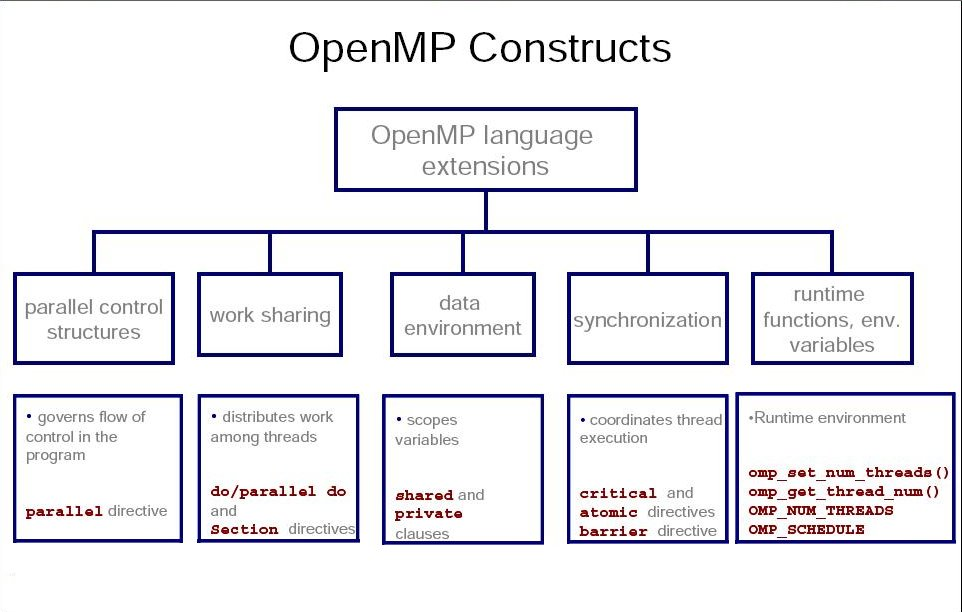
\includegraphics[width=0.8\textwidth,height=0.6\textheight,keepaspectratio]{img/openmp.jpg}
  \end{center}
\end{frame}



\begin{frame}
  \frametitle{MPI}

  \begin{itemize}
  \item Message Passing Interface
  \item Process based parallel computing API
  \item Targeted to clusters
  \item Feature rich
    \begin{itemize}
    \item Message passing
    \item Synchronization
    \item Data sharing
    \item I/O
    \end{itemize}
  \end{itemize}
\end{frame}
